\chapter{Theoretical Framework}


\section{Gravitational Waves Theory}
After considering, in 1905, the problem of the apparently \textit{instantaneous} propagation of light, with the theory of Special Relativity, in 1916 Albert Einstein considered the problem of the apparently \textit{instantaneous} propagation of gravity through \textit{long distances}, in his theory of General Relativity.
Einstein showed that long-distance interaction arises from the deformation of space time caused by massive objects.
Hence, in the "static case", the deviated motion apparently caused by the interaction between two distant masses really is, in fact, a manifestation of space time curvature nearby, generated by the presence of the two objects.
The "static case" just depicted, though, treats the curvature as if it had always been there, and doesn't take into account of any variation in the masses, positions or velocities of the two objects, that would induce an evolution to the curvature itself.
In truth, after a change in the mass-energy distribution, the corresponding curvature variation requires its time to reach far distances, and a fascinating prediction of General Relativity is that it propagates in the form of a wave, that travels at the speed of light.
\subsection{Gravitational Waves as Perturbations}
The typical approach to the study of gravitational waves is to derive them as small perturbations of the background from the Einstein's equations: 
\begin{equation}
    G_{\mu\nu} = R_{\mu\nu} - \frac{1}{2}g_{\mu\nu}R,
\end{equation}
which can be conveniently written as 
\begin{equation}
    R_{\mu\nu}=\frac{8\pi G}{c^4}\left(T_{\mu\nu} - \frac{1}{2}g_{\mu\nu}T\right),
    \label{eq: Einstein equations rewritten}
\end{equation}
where $G_{\mu\nu}$ is the Einstein tensor, $R_{\mu\nu}$ is the Ricci tensor, $R$ is the Ricci scalar, $g_{\mu\nu}$ is the metric of space time, and $T_{\mu\nu}$ is the stress-energy tensor.
As a background solution we can consider the flat space time described by the metric $\eta_{\mu\nu}$, to which the perturbation term appears as a fluctuation in the metric $|h_{\mu\nu}|\ll|\eta_{\mu\nu}|$, known as \textit{weak field} approximation. Thus, the perturbed space time can be written as:
\[
    g_{\mu\nu} = \eta_{\mu\nu} + h_{\mu\nu}, \hspace{5mm}  |h_{\mu\nu}|\ll|\eta_{\mu\nu}|.
\] 
With this metric, the equations \ref{eq: Einstein equations rewritten} becomes
\[
    \{\square_F h_{\mu\nu} - \left[\frac{\partial^2}{\partial x^\lambda\partial x^\mu}h^\lambda_\nu + \frac{\partial^2}{\partial x^\lambda\partial x^\nu}h^\lambda_\mu + \frac{\partial^2}{\partial x^\nu\partial x^\mu}h^\lambda_\lambda\right]\} = -\frac{16\pi G}{c^4}\left(T_{\mu\nu} - \frac{1}{2}\eta_{\mu\nu}T\right).
\]
Now, by requiring that the \textit{weak-field} approximation remains satisfied for infinitesimal diffeomorphisms, and by choosing a coordinate system in which the \textit{harmonic gauge condition}\footnote{It is an arbitrary coordinate condition which makes it possible to solve the Einstein field equations. It can be found by requiring that the linearized Einstein equations satisfy the D'Alambert equation.}, defined as 
\begin{equation}
    \Gamma^\lambda = g^{\mu\nu}\Gamma^\lambda_{\mu\nu} = 0,
    \label{eq: Harmonic gauge definition}
\end{equation}
where $\Gamma^\lambda_{\mu\nu}$ are the \textit{affine connections}, is satisfied, we can find that, up to first order in $h_{\mu\nu}$, the harmonic gauge condition is equivalent to 
\begin{equation}
    \frac{\partial}{\partial x^\mu}h^\mu_\rho = \frac{1}{2}\frac
    {\partial}{\partial x^\rho}h, \hspace{5mm} h=\eta^{\mu\nu}h_{\mu\nu}\equiv h^\nu_\nu.
\end{equation}
After defining the \textit{trace-reversed}\footnote{The name comes by noting that $\bar{h}=\eta^{\mu\nu}\bar{h}_{\mu\nu} = -h$.} tensor as
\begin{equation*}
    \bar{h}_{\mu\nu} \equiv h_{\nu\mu} - \frac{1}{2}\eta_{\mu\nu}h,
\end{equation*}
we can finally write the linearized Einstein equations as
\begin{equation}
    \left\{
        \begin{aligned}
            \square\bar{h}_{\mu\nu} &= -\frac{16\pi G}{c^4} T_{\mu\nu}, 
            \notag\\
            \partial^\mu \bar{h}_{\mu\nu} &= 0.
        \end{aligned}
    \right.
    \label{eq: Einstein equations as wave equations}
\end{equation}
This form, and its twin with $T_{\mu\nu}=0$, where the first equation becomes the D'Alambert equation, are relevant because they show that \textit{a perturbation of a flat space time propagates as a wave travelling at the speed of light}.
As in Electrodynamics, the solution of~\eqref{eq: Einstein equations as wave equations} can be written in terms of \textit{retarded potentials}:
\begin{equation}
    \bar{h}_{\mu\nu}(t,\mathbf{x}) = \frac{4G}{c^4}\int_V \frac{T_{\mu\nu}(t - \frac{|\mathbf{x} - \mathbf{x}'|}{c}, \mathbf{x}')}{|\mathbf{x} - \mathbf{x}'|}d^3x',
    \label{eq: solutions with retarded potentials}
\end{equation}
where V is the three dimensional source volume, $\mathbf{x}'$ is the distance of an element of the emitting source from the origin of a frame centered in the same point of the source, $\mathbf{x}$ is the distance between source and observer.
It can be proved that the solutions in \eqref{eq: solutions with retarded potentials} automatically satisfy the harmonic gauge condition in the second equation of the \eqref{eq: Einstein equations as wave equations}.


\subsubsection{Harmonic gauge}
It is important to notice that if the \textit{harmonic gauge} condition is not satisfied in a reference frame, a new frame in which it is can always be found, by making an infinitesimal coordinate transformation
\begin{equation}
    x^{\lambda'} = x^\lambda + \epsilon^\lambda,
    \label{eq: infinitesimal coordinate transformation}
\end{equation}
provded that $\epsilon^\lambda$ satisfies the following equation:
\[
    \square_F\epsilon_\rho = \frac{\partial h^\beta_\rho}{\partial x^\beta} - \frac{1}{2} \frac{\partial h}{\partial x^\rho} = 0\hspace{1mm}.
\]
This is an inhomogeneous wave equation that can be solved to find the components $\epsilon_\alpha$, which identify the coordinate system in which the harmonic gauge condition is satisfied.
Notice though, that the harmonic condition in \eqref{eq: Harmonic gauge definition} does not determine the gauge uniquely, but instead leaves some more gauge freedom to be used.

\subsection{The physical wave}
As we have seen, perturbations of flat space-time satisfy a wave equation and a harmonic gauge condition, as in \eqref{eq: Einstein equations as wave equations}.
The general solutions of these wave equation is a linear superposition of monochromatic plane waves, with a polarization tensor (or wave amplitude) $A_{\mu\nu}$ and a wave four-vector $\vec{k}$, such as
\[
    \square_F \bar{h}{\mu\nu} = -A_{\mu\nu}\eta^{\alpha\beta} k_\alpha k_\beta e^{ik_\gamma x^\gamma} = 0.
\]
Thus, neglecting the trivial solution $A_{\mu\nu} = 0$, gives 
\[
    \eta^{\alpha\beta} k_\alpha k_\beta = 0,
\]
which means that $\vec{k}$ is a null vector.
If we also consider the harmonic gauge, we find a condition that imposes the orthogonality  of the wave four-vector to the polarization tensor,
\[
    k_\mu A^\mu_\nu = 0.
\]
The \textit{wavefronts}, i.e. the spatial surfaces where $\bar{h}_{\mu\nu}= const.$ are the planes where $k_ix^i=const.$
Conventionally, $k^0$ is referred to as $\frac{\omega}{c}$, where $\omega$ is the frequency, thus
\[
    \vec{k}_0 = \left(\frac{\omega}{c},\mathbf{k}\right),
\]
where $\mathbf{k}$ is the wave three-vector orthogonal to the wavefront, and is related to the \textit{wavelenght} by $|\mathbf{k}| = 2\pi/\lambda$.
Notice that, since the wave four-vector $\vec{k}$ is a null vector, it follows that
\[
    -(k^0)^2 + |\mathbf{k}| = 0 \to \omega = ck_0 = c|\mathbf{k}|,
\]
which gives the dispersion relation for a wave moving at the speed of light.


\subsubsection{The TT gauge}
In a one dimension case, the wave equation can be written as
\[
    \left( -\frac{1}{c^2} \frac{\partial^2}{\partial t^2}  + \frac{\partial^2}{\partial x^2}\right)\bar{h}^\mu_\nu = 0,
\]
which generally has, as solution, an arbitrary function of $t\pm \frac{x}{c}$.
If we consider, for example, a progressive wave $\bar{h}^\mu_\nu [f(t,x)]$, where $f(t,x) = t- \frac{x}{c}$, and apply the harmonic gauge condition, focusing only in the time-depndent part of the solution, we find the \textit{first four} conditions:
\begin{equation}
    \bar{h}^t_t = \bar{h}^x_t, \hspace{5mm} \bar{h}^t_x = \bar{h}^x_x, \hspace{5mm} \bar{h}^t_y = \bar{h}^x_y, \hspace{5mm} \bar{h}^t_z = \bar{h}^x_z.
    \label{eq: first four conditions}
\end{equation}
As we have already discussed, there still is the freedom of making an infinitesimal coordinate change, and by requiring that the harmonic gauge remains satisfied in the new coordinates generates \textit{four more conditions}:
\begin{equation}
    \bar{h}^t_x = \bar{h}^t_y = \bar{h}^t_z = \bar{h}^y_y + \bar{h}^z_z = 0,
    \label{eq: second four conditions}
\end{equation}
and with the~\eqref{eq: first four conditions} follows
\[
     \bar{h}^x_x = \bar{h}^x_y = \bar{h}^x_z = \bar{h}^t_t = 0.
\]
The only non zero components are $\bar{h}^z_y$ and $\bar{h}^y_y - \bar{h}^z_z$, which cannot be set to zero because now we have completely used all the gauge freedom.
It can be shown that, from all the above conditions, it follows that $\bar{h} \equiv h$, i.e. in this gauge the wave results to be \textit{traceless}.
Thus, a plane gravitational wave propagating along the $x$-axis is characterized by only two non-zero functions $h_{zy}$ and $h_{yy}=-h_{zz}$:
\begin{equation}
    h^{TT}_{\mu\nu} =  
    \begin{pmatrix}
0 & 0 & 0 & 0 \\
0 & 0 & 0 & 0 \\
0 & 0 & h_{yy} & h_{yz} \\
0 & 0 & h_{yz} & -h_{yy}
\end{pmatrix}.
    \label{eq: h as a matrix in x case}
\end{equation}
In conclusion, the gravitational wave only has \textbf{two physical degrees of freedom} which correspond to two polarization states.
This gauge is called \textbf{TT gauge} because of the \textit{transverse traceless} nature: $h_{\mu\nu}$ is traceless, thus $h=0$, and transverse, since the components of $h_{\mu\nu}$ along the direction of propagation are null (in this case $h_{\mux}=0$).

\subsection{Motion and geodesics}
Free test particles in General Relativity move along geodesic, which means that, in terms of a world line $x^\mu(\tau)$ parametrized by proper time $\tau$, they satisfy the \textit{geodesic equation}:
\begin{equation}
    \frac{d^2x^\alpha}{d\tau^2} + \Gamma^\alpha_{\mu\nu} \frac{dx^\mu}{d\tau}\frac{dx^\nu}{d\tau} \equiv \frac{du^\alpha}{d\tau} + \Gamma^\alpha_{\mu\nu}u^\mu u^\nu = 0,
    \label{eq: geodesic equation of free particle}
\end{equation}
where $u^\alpha = \frac{dx^\alpha}{d\tau}$ is the particle velocity.
By imposing the rest condition, $u^\alpha = (1,0,0,0)$, to the~\eqref{eq: geodesic equation of free particle} and considering the TT gauge component prescriptions for $h_{\mu\nu}$, we find that a particle initially at rest is not accelerated by the passage of a wave, but remains at a fixed coordinate position: the motion of a single particle is not affected by the gravitational waves.

\subsubsection{The geodesic deviation}
If we consider, instead, the relative motion of close particles, the situation is different.
This relative motion is governed by the \textit{geodesic deviation}, which quantifies how two very close geodesics deviate from one another.
Although, as we have seen, the coordinates of the two particles (and thus their difference) do not change when a gravitational wave passes, this does not hold true for their \textit{proper distance} o
\[
    \Delta l = \int ds \not = const.
\]
This apparent contradiction arises from the fact that the coordinate difference is not a \textit{tensorial} quantity, and therefore is not suited to describe properly a physical process.
This is the reason we consider the geodesic deviation, which provides a tensorial formulation of the relative acceleration between the two particles: 
\begin{equation}
    \frac{D^2\delta x^\alpha}{d\tau^2} \equiv (\Delta_{\vec{t}}(\Delta_{\vec{t}}\vec{\delta x}))^\alpha = R^\alpha_{\beta\mu\nu}t^\beta t^\mu \delta x^\nu,
    \label{eq: geodesic deviation}
\end{equation}
where 
\begin{equation}
    R_{\alpha k \lambda \mu} = \frac{1}{2}( g_{\alpha\mu,\lambda k}  + g_{k\lambda,\mu \alpha }  - g_{\alpha\lambda,\mu k }  - g_{k\mu,\lambda \alpha })
    \label{eq: Riemann tensor def}
\end{equation}
is the Riemann curvature tensor, $\vec{t}$ is the tangent vector to one of the geodesic, and $\vec{\delta x}$ is a deviation vector between the two geodesics.
it is important to note that in the presence of a gravitational wave the Riemann tensor is never zero in any reference frame, and consequently neither is the geodesic deviation. 
In contrast, the quantity $\frac{d^2\delta x^i}{d\tau^2}$ (which is not a tensorial quantity) vanishes in the TT frame.

Knowing this, to analyze this effect in more detail we can choose to integrate the~\eqref{eq: geodesic deviation} in a \textit{Locally Inertial Frame}, LIF \{$\xi^\alpha$\}, centered on one of the two particles, where the metric can be approximated close to the origin as Minkowski up to quadratic, negligible, corrections:
\[
    ds^2 = \eta_{\alpha\beta} d\xi^\alpha d\xi^\beta + O(|\xi|^2).
\]
In this frame, the Riemann tensor in~\eqref{eq: Riemann tensor def}, which depends on second derivatives of the metric perturbation $h_{\mu\nu}$ (with $g_{\mu\nu} = \eta_{\mu\nu} + h_{\mu\nu}$), is not only covariant, but actually \textit{invariant} under infinitesimal coordinate transformations from a generic LIF to the TT frame. 
This is especially useful because in the TT frame $h^{TT}_{\mu\nu}$ takes a particularly simple form, as we have seen in the~\eqref{eq: h as a matrix in x case} example, simplifying also the expression for $R^{TT}_{\alpha k \lambda \mu$. 
Assuming that the wave travels along the $\xi^1$ direction, the solutions for the geodesic deviation equation for two close particles are the non zero components of 
\begin{equation}
    \delta\xi^j = \delta\xi_0^j + \frac{1}{2}\eta^{ji} h^{TT}_{ik} \delta\xi_0^k,
    \label{eq: solution of geodesic deviation}
\end{equation}
where $\delta\xi_0^j$ represent the initial, constant separaion between the particles. 
As previously discussed, the non-zero components of the strain tensor $h_{ik}^{TT}$ correspond to two possible polarizations of the gravitational wave. 
Their distinct effects on a ring of close particles are viually represented in \textbf{Figure~\ref{fig:gw_polarizations}}.
\begin{figure}[h]
    \centering
    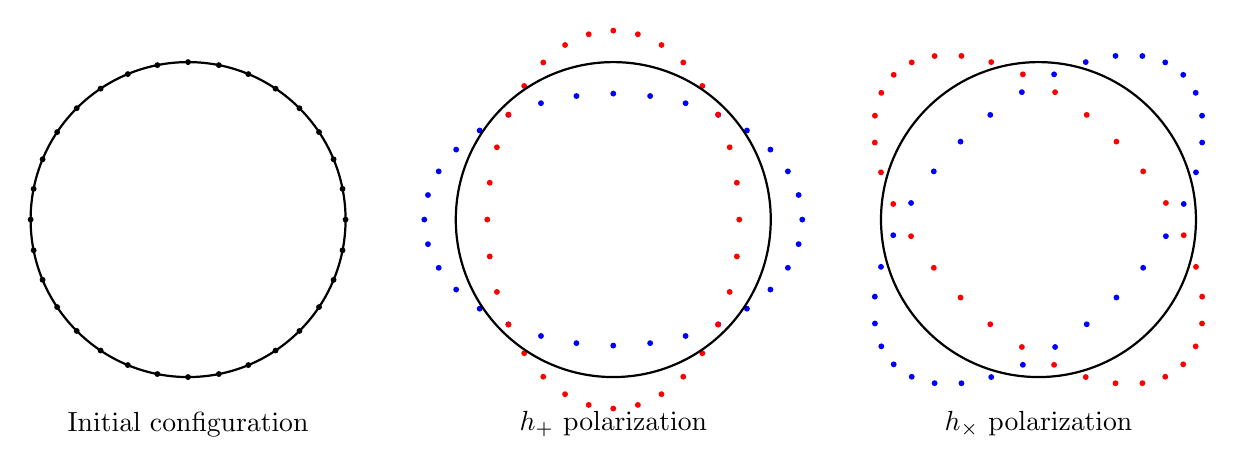
\begin{tikzpicture}[scale=2]

    % Configurazione iniziale (cerchio)
    \foreach \angle in {0,11.25,...,348.75}{
        \node[circle,fill=black,inner sep=0.75pt] at (\angle:1) {};
    }
    \draw[thick] (0,0) circle(1);
    \node at (0,-1.3) {Initial configuration};

    % Polarizzazione +
    \begin{scope}[xshift=2.7cm]
        % Fase 1: ellisse orizzontale
        \foreach \angle in {0,11.25,...,348.75}{
            \pgfmathsetmacro{\x}{cos(\angle)}
            \pgfmathsetmacro{\y}{sin(\angle)}
            \node[circle,fill=black,inner sep=0.75pt,blue]
                at ({1.2*\x},{0.8*\y}) {};
        }
        % Fase 2: ellisse verticale
        \foreach \angle in {0,11.25,...,348.75}{
            \pgfmathsetmacro{\x}{cos(\angle)}
            \pgfmathsetmacro{\y}{sin(\angle)}
            \node[circle,fill=black,inner sep=0.75pt,red]
                at ({0.8*\x},{1.2*\y}) {};
        }
        % Cerchio di riferimento
        \draw[thick] (0,0) circle(1);
        \node at (0,-1.3) {${h}_{+}$ polarization};
    \end{scope}

    % Polarizzazione ×
    \begin{scope}[xshift=5.4cm]
        % Fase 1: shear a +45°
        \foreach \angle in {0,11.25,...,348.75}{
            \pgfmathsetmacro{\x}{cos(\angle)}
            \pgfmathsetmacro{\y}{sin(\angle)}
            \pgfmathsetmacro{\xp}{\x + 0.3*\y}
            \pgfmathsetmacro{\yp}{\y + 0.3*\x}
            \node[circle,fill=black,inner sep=0.75pt,blue] at (\xp,\yp) {};
        }
        % Fase 2: shear a -45°
        \foreach \angle in {0,11.25,...,348.75}{
            \pgfmathsetmacro{\x}{cos(\angle)}
            \pgfmathsetmacro{\y}{sin(\angle)}
            \pgfmathsetmacro{\xp}{\x - 0.3*\y}
            \pgfmathsetmacro{\yp}{\y - 0.3*\x}
            \node[circle,fill=black,inner sep=0.75pt,red] at (\xp,\yp) {};
        }
        % Cerchio di riferimento
        \draw[thick] (0,0) circle(1);
        \node at (0,-1.3) {${h}_{\times}$ polarization};
    \end{scope}

    \end{tikzpicture}
    \caption{Effect of the two gravitational wave polarizations on a ring of free-falling particles: blue and red dots represent two opposite phases of the wave.}
    \label{fig:gw_polarizations}
\end{figure}



\subsection{The Quadrupole Approximation}
\subsubsection{The weak-field, slow-motion approximation}
\subsubsection{The quadrupole formula}
\subsubsection{Transform to the TT gauge}

\subsection{Gravitational waves from a binary system}
\subsubsection{General solution for circular orbits}
Up to 13.86/7 at page 255 of the book.

\subsection{Energy carried by a gravitational wave}
\subsubsection{Stress-energy pseudo-tensor}
\subsubsection{Gravitational wave luminosity}

\subsection{Evolution of a compact binary system}
\subsubsection{Signal from inspiralling compact objects}
Here we get to the actual amplitude we used, and the parameters involved.

\section{White dwarfs and galaxies}
\subsection{White dwarfs}
\subsection{Galaxies}
\subsubsection{Morphological types}
Here I introduce Hubble types, explaining general physical differences between them.
Later I will introduce the T value notation and how to translate in the Hubble sequence types. 

\section{LISA}
\section{interferometers}



- Instrument description (what is an interferometer, why in space, how it will be made, orbit)
- frequency band - what will it see?
- frequency resolution
- sensibility curve and ASD meaning
- Why WD choice in particular?

